\chapter{Project Overview}

\section{Background and Motivation}

Climate change is a growing concern due to the effects that global warming has on the environment. As the population of the world increases, the energy demand will increase in turn. Due to the reliance on fossil fuels, this will only increase the amount of greenhouse gases that is produced into the atmosphere. This is why it is important to explore alternative energies that are relatively “greener” in comparison to the standard fossil fuels that are mainly used.

\medskip
A major sector where energy can be saved is domestic hot water heating. 19.3\% of the residential energy usage in Canada is from water heating \cite{water_heaters}. This statistic can be improved with the implementation of technology that uses other sources of energy to provide water heating. This project focuses on a Direct Expansion Solar Assisted Heat Pump (DX-SAHP), which is an example of a technology that can be used in place of natural gas for heating. The DX-SAHP combines the benefits of a heat pump with the abundance of solar energy that we receive.

\medskip
Unlike an Air Source Heat Pump (ASHP), the DX-SAHP uses a combination of solar energy and the ambient temperature to evaporate the refrigerant, improving the performance and making it viable for areas with a colder climate. The use of solar energy in conjunction with the heat pump reduces the amount of electricity that is needed for a standard heat pump to generate hot water.

\newpage
\begin{figure}[ht]
    \centering
    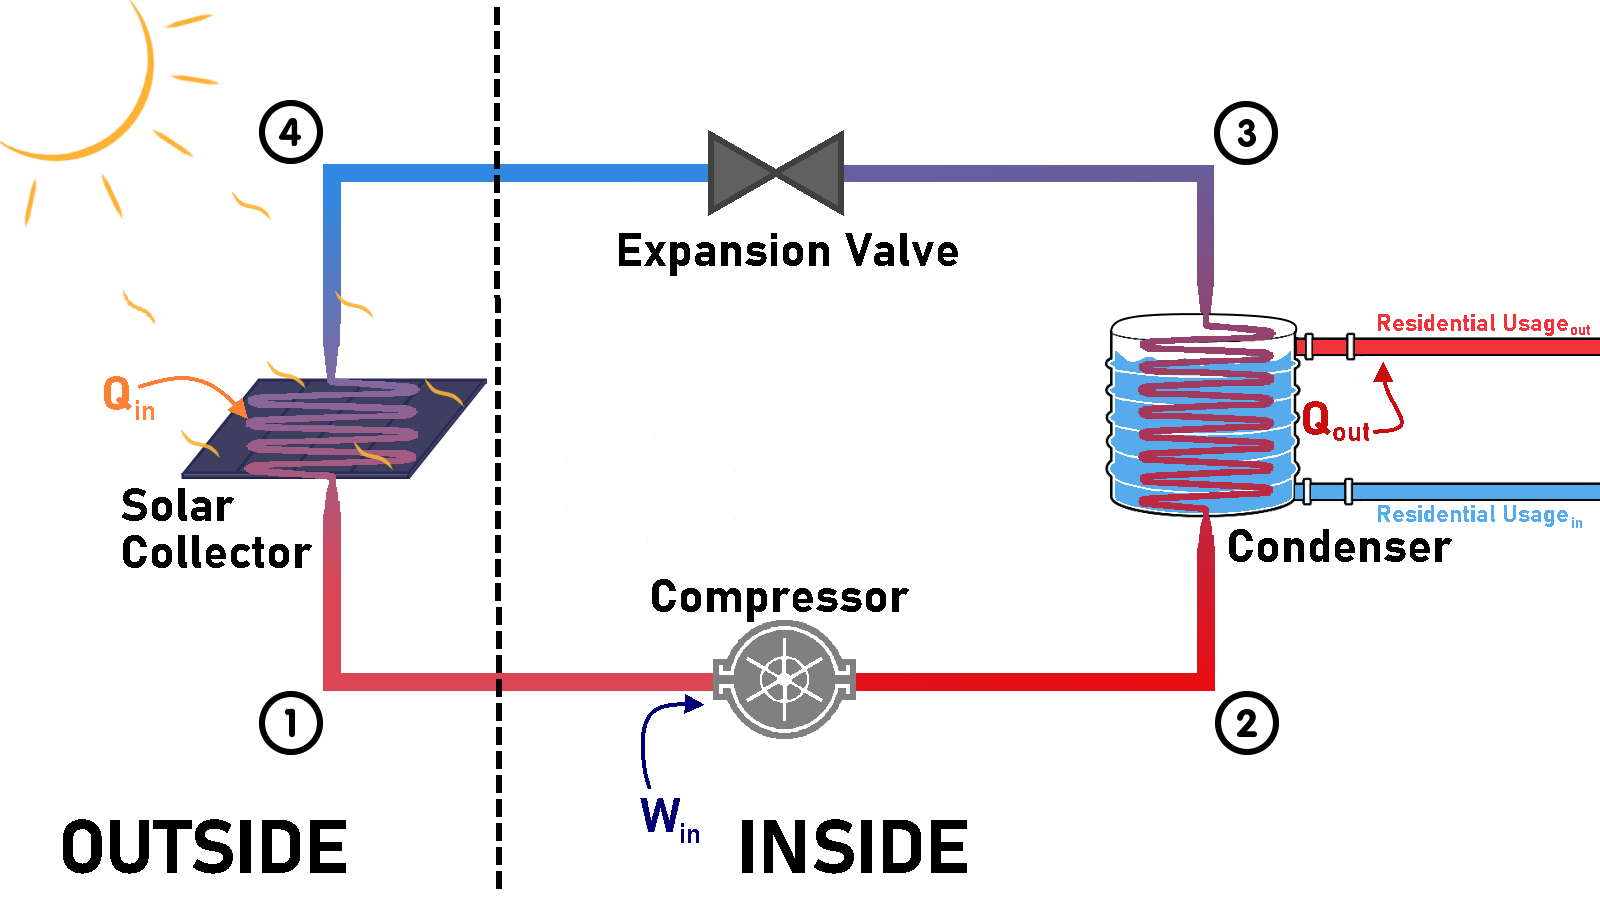
\includegraphics[width=\textwidth]{images/schematic.png}
    \caption{DX-SAHP Schematic}
\end{figure}
\medskip
The solar collector is what will be used instead of a traditional evaporator in the DX-SAHP. The collector is heated up, due to it being in direct sunlight, and thus it heats up and evaporates the refrigerant running below it. Ambient temperatures play a critical role in the performance of a heat pump with a solar collector. This is due to the solar collector directly being affected by how much irradiance, the amount of light striking a surface, is available. To design a collector for colder climates, where perhaps less irradiance is available, there must be key considerations that are considered. Additionally, other required components must be matched to the demand and to the solar collector size.

\section{Problem Statement}
The current state of heating in Alberta is overly reliant on natural gas and the technology that is currently being used to heat domestic water is contributing to the increase in global temperatures via greenhouse gas emissions. DX-SAHP can be used to phase out natural gas heaters by using the sun as an energy source instead. Therefore, a DX-SAHP can be designed that can heat an average household of 3 people within the Calgary region.

\section{Overview of Scope}
The goal of this capstone is to design a DX-SAHP that can heat 225L of domestic hot water to a household of 3 people. This number was calculated from the information from the Government of Canada stating that the average Canadian uses 75L of hot water a day \cite{water_heaters}. Knowing this, a DX-SAHP will be designed and manufactured. The effort will be mainly focused on optimizing the area of the collector while reducing the heat losses from convection and radiation. Component matching analysis and selecting a compatible compressor, condenser, and electronic expansion valve is necessary so that it is system functions properly. This heat pump must be equipped with all the necessary controls and data acquisition systems. Afterwards a working model will be made in order to be functional within Calgary and an economic and environmental analysis will be conducted to justify the proposed system.

\medskip
To determine the sizing of the DX-SAHP initial parameters must be set.

\medskip
Statistics Canada states that the average Canadian household occupies 2.47 members, and the average Canadian uses 75L of hot water per day \cite{stats_canada}. For the purposes of the DX-SAHP, it will be assumed that a domestic household of 3 people will require 225L of hot water per day. The hot water will be required to exit the system at a temperature of 50\textdegree C for residential use to avoid bacteria buildup in the water tank such as legionella. 

\medskip
The municipal water supply differs in temperature depending on the time of year. When it is winter, municipal line comes in at 10\textdegree C unlike in the summer when it comes in at 20\textdegree C. This is an important parameter to be considered when quantifying what heat load the heat pump will have to supply.

\medskip
To validate and maintain quantifiable design goals, the project will be considered successful if it is able to sustain 225L of water at 50\textdegree C while maintaining a coefficient of performance ($COP$) greater than 2.3. This means the DX-SAHP must be able to provide the following heat loads.

\smallskip
\begin{align}
    Q_L = 225L \times \frac{1000g}{1L} \times 4.18\frac{J}{g\SI{}{\celsius}}\times (\SI{50}{{\celsius}} - \SI{10}{{\celsius}}) = 37,620kJ
    \\\eqname{Heat Load Required during Winter Conditions}
\end{align}

\begin{align}
    Q_L = 225L \times \frac{1000g}{1L} \times 4.18\frac{J}{g\SI{}{\celsius}}\times (\SI{50}{\celsius} - \SI{20}{\celsius}) = 28,215kJ
    \\\eqname{Heat Load Required during Summer Conditions}
\end{align}
